\chapter{Results} \label{chap:experiments}

This Chapter describes the experiments done in this work and the results achieved.

\section{Data}
Two datasets were used in the experiments, our collected dataset HuPBA-AgeGuess and the classic benchmark database FG-NET.

\textbf{FG-NET} consists of 1002 frontal face images of 82 different individuals. The image quality varies a lot in the dataset since there are images in grey scale and RGB. The face position is frontal and under similar illumination conditions. The dataset also contain 68 facial landmarks for each face image.

\begin{figure}[!h]
	\centering
	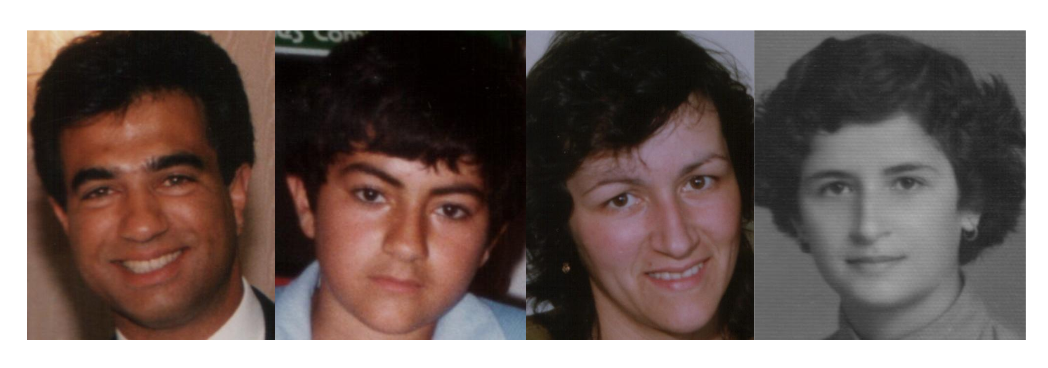
\includegraphics[width=\textwidth]{figures/FGNET_sample}
	\caption{FG-NET image samples.}
	\label{fig:imgSample1}
\end{figure}

\textbf{HuPBA-AgeGuess} dataset (\ref{fig:imgSample2}) used in this project is a subset of the 4865 images filtered out by a minimum number of votes per image. This subset contains 3398 face images. The images are captured in the wild so the faces position vary up to $\pm90º$ and the illumination is also different in every picture.

\begin{figure}[!h]
	\centering
	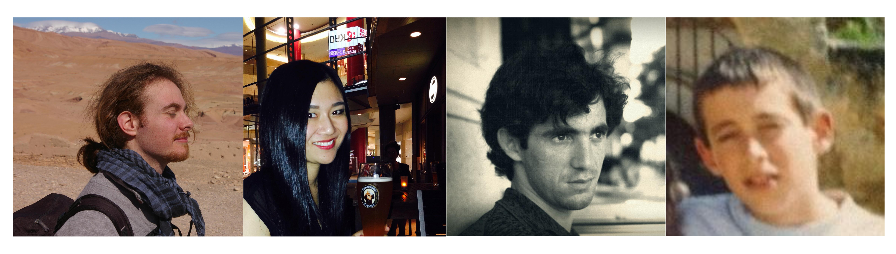
\includegraphics[width=\textwidth]{figures/HuPBA_sample}
	\caption{HuPBA-AgeGuess image samples.}
	\label{fig:imgSample2}
\end{figure}

\section{Methods and Parameters}

\section{Experimental Settings}
This Section describes the experimental setup 
\subsection{Evaluation Metrics} 

The two most commonly used evaluation metrics in age estimation are Mean Absolute Error (MAE) and Cumulative Score (CS).

The MAE is described as

\begin{equation}
MAE = \frac{1}{n}\sum_i^{n} |e_i|
\end{equation}

where $e_i$ is the error of the $ith$ instance, i.e. $e_i = |\hat{y_i} - y_i|$ where $y_i $ is the real label and $\hat{y_i}$ is the predicted label. This metric tells the average number of years that the prediction is wrong.

CS is defined as the percentage of test images such that the absolute error is not higher than a threshold, $t$ (in years). i.e.,

\begin{equation}
CS(t) = (1 - \frac{1}{n}\sum_i^n h(|\hat{y_i} - y_i| - t))\cdot 100
\end{equation}
\begin{equation}
h(x) = 
\begin{cases}
1,				& \text{if } x \geq 0\\
0,              & \text{otherwise}
\end{cases}
\end{equation}

where $y_i$ is the age label of the $ith$ test image and $\hat{y_i}$ is the age prediction of the $ith$ test image.

\section{Experiments}

\begin{figure}[!h]
	\centering
	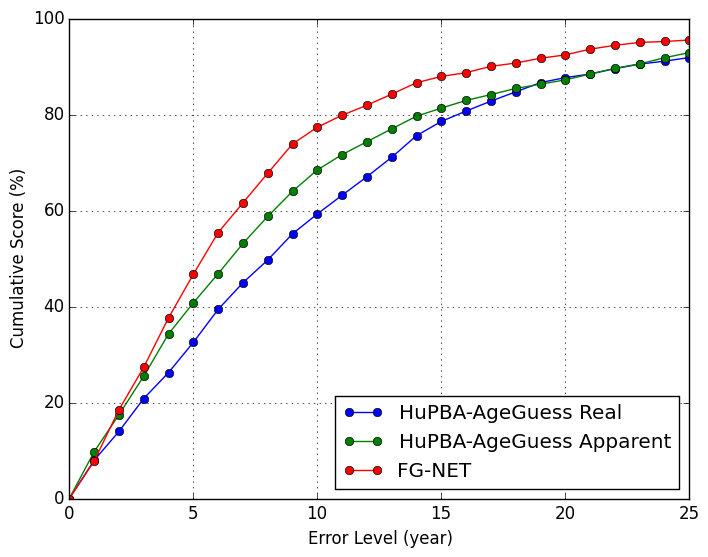
\includegraphics[width=\textwidth]{figures/cum_score}
	\caption{Cummulative Score }
	\label{fig:cumS}
\end{figure}
